\documentclass[12pt]{article}

\usepackage[top=0.75in,bottom=0.75in,left=0.5in,right=0.5in]{geometry}
\usepackage{amsmath,amssymb,multirow,graphicx}
\usepackage{wrapfig}

\newcommand{\bee}[1]{\begin{equation} #1 \end{equation}}
\newcommand{\baa}[1]{\begin{eqnarray} #1 \end{eqnarray}}
\newcommand{\bees}[1]{\begin{equation*} #1 \end{equation*}}
\newcommand{\baas}[1]{\begin{eqnarray*} #1 \end{eqnarray*}}

\newcommand{\pd}[2]{\ensuremath{\frac{\partial #1}{\partial #2}}}
\newcommand{\dd}[2]{\ensuremath{\frac{d #1}{d #2}}}

\newcommand{\bx}{{\mathbf x}}
\newcommand{\ba}{{\mathbf a}}
\newcommand{\bl}{{\pmb \ell}}
\newcommand{\bu}{{\mathbf u}}
\newcommand{\bv}{{\mathbf v}}
\newcommand{\bq}{{\mathbf q}}
\newcommand{\ff}{{\mathbf f}}
\newcommand{\bS}{{\mathbf S}}
\newcommand{\bI}{{\mathbf I}}
\newcommand{\bA}{{\mathbf A}}
\newcommand{\bG}{{\mathbf G}}
\newcommand{\bF}{{\mathbf F}}
\newcommand{\bP}{{\mathbf P}}
\newcommand{\bQ}{{\mathbf Q}}
\newcommand{\bU}{{\mathbf U}}

\newcommand{\pe}{\phi_\epsilon}
\newcommand{\Ge}{G_\epsilon}
\newcommand{\Be}{B_\epsilon}
\newcommand{\eps}{\epsilon}

\title{Regularized Stokeslet Derivation in 2D: A Cubic Blob}
\author{Bree Cummins and John Chrispell}


\begin{document}

\maketitle

We solve the 2D Stokes equations with a regularized point force located at $\bx_0$:
\bees{
\mu\nabla^2 \bu = \nabla p - \ff \pe(\bx - \bx_0), \qquad \nabla \cdot \bu = 0
}
with the specific blob function 
\bees{
\pe(r) = \frac{2\eps^4}{\pi(r^2 + \eps^2)^3}
}
where $r = |\bx - \bx_0|$ and $\eps$ is a small, positive parameter. From Ricardo's work, we know that given the solutions to 
\bee{
\nabla^2 \Ge(r) = \pe(r) \text{ and } \nabla^2 \Be(r) = \Ge(r), \label{eqn:poisson}
}
we may write the solution to the Stokes equations as 
\bees{
\mu\bu(\bx) = \left(\ff \cdot \nabla \right)\nabla \Be(r) - \ff\Ge(r).
}
Because of the spherical symmetry, this equation may be rewritten as 
\bee{
\mu\bu(\bx) = \left( \frac{\Be'(r)}{r} - \Ge(r)\right)\ff + \big[\ff \cdot (\bx -\bx_0)\big](\bx -\bx_0)\frac{r\Be''(r) - \Be'(r)}{r^3}, \label{eqn:usoln}
}
where the primes denote differentiation with respect to $r$.

Our goal is to find the functions $\Ge$ and $\Be$. We solve the two Poisson equations in Eq.~\eqref{eqn:poisson} by first changing to polar coordinates:
\baas{
\frac{1}{r}\left( r \Ge'(r) \right)' &=& \frac{2\eps^4}{\pi(r^2 + \eps^2)^3} \\
r \Ge'(r) &=& \int \frac{r 2\eps^4}{\pi(r^2 + \eps^2)^3} dr.
}
\pagebreak 

Now do a $u$ substitution. Let
\bee{
u = r^2 + \eps^2, \quad du = 2r dr, \label{eqn:usub}
}
then
\baas{
r \Ge'(r) &=& \int \frac{\eps^4 du}{\pi u^3} \\
&=& \frac{\eps^4}{\pi} \left(\frac{u^{-2}}{-2} \right) + C\\
&=& \frac{-\eps^4}{2\pi} \frac{1}{(r^2 + \eps^2)^2} + C \\
\Ge(r) &=& \frac{-\eps^4}{2\pi} \int \frac{dr}{r(r^2 + \eps^2)^2} + C \int \frac{dr}{r}.
}


\begin{wrapfigure}[4]{l}{2.25in}
	\begin{center}
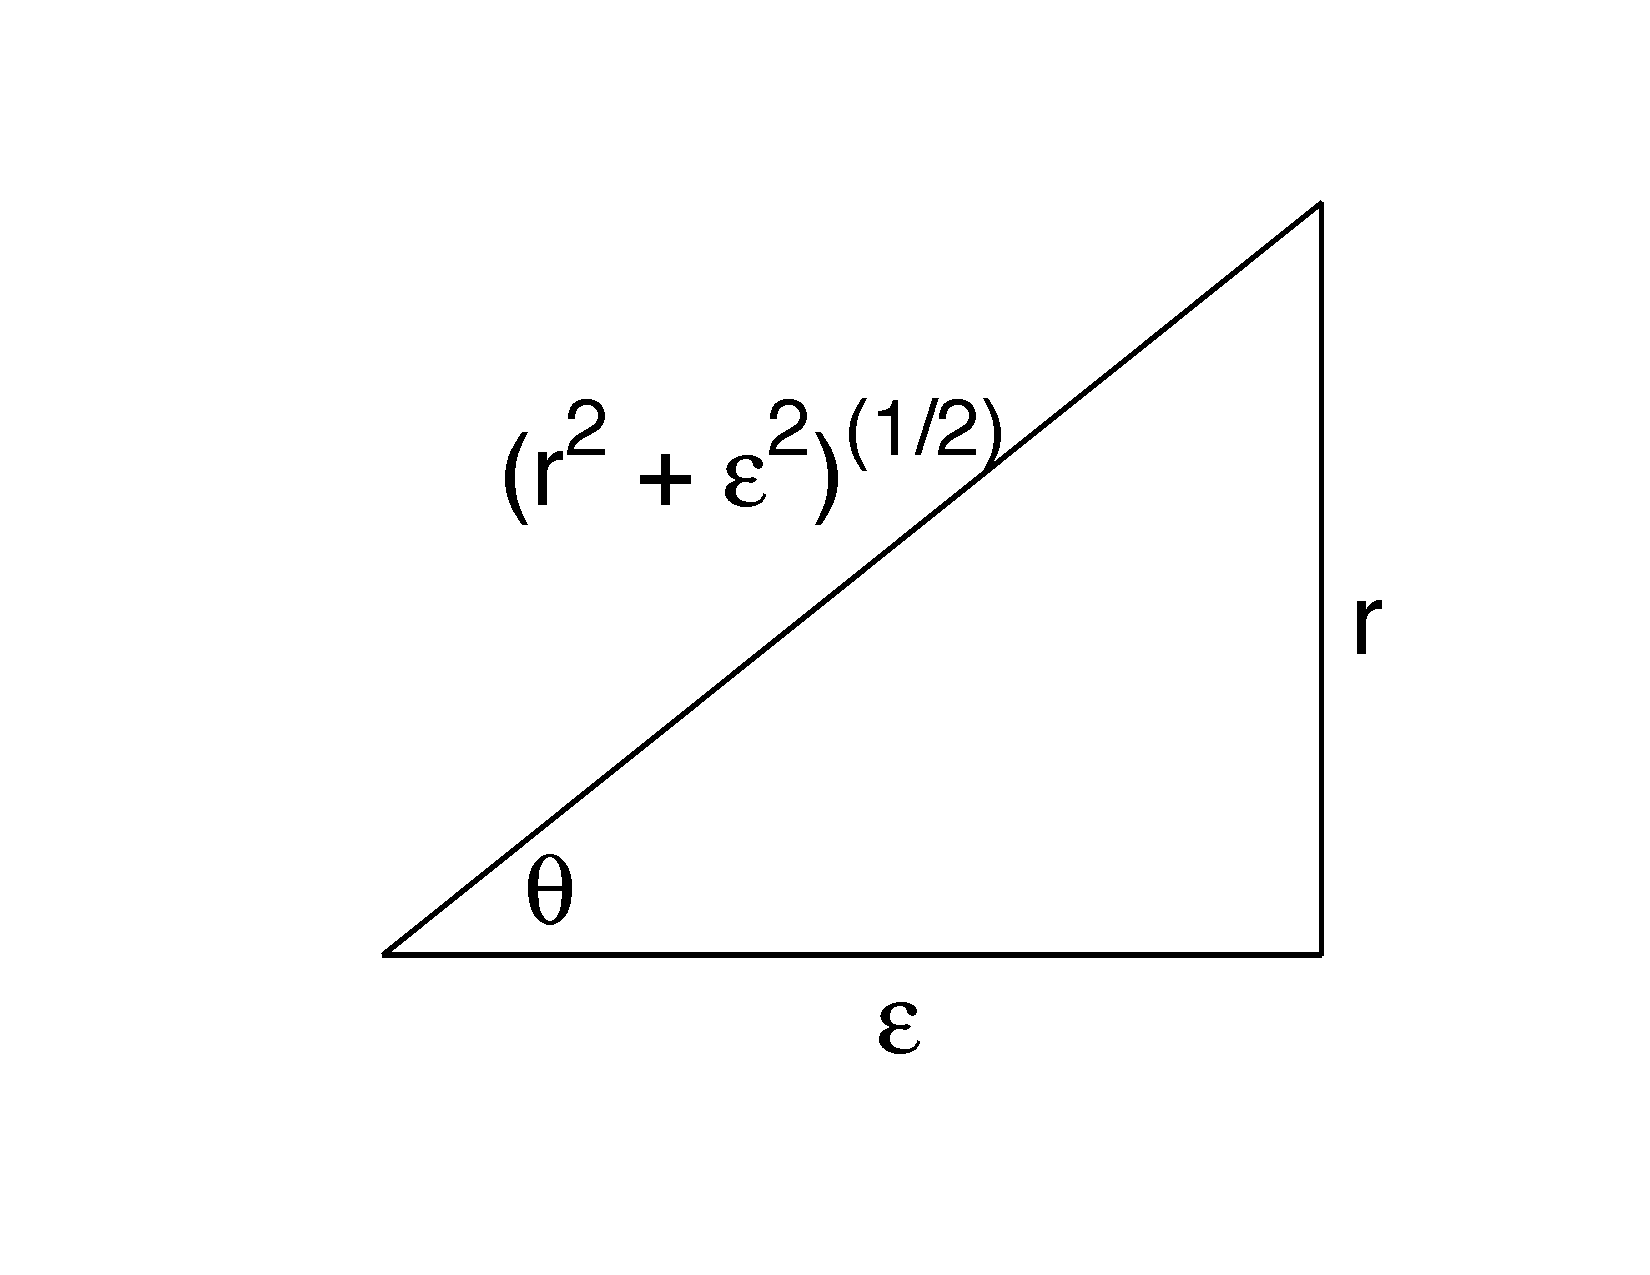
\includegraphics[width=2.0in]{TrigSubsTriangle.pdf}
\end{center}
%\caption{Triangle from trig substitution.}
\end{wrapfigure}
Trig substitution: Let $\eps\tan\theta = r, \eps\sec^2\theta \;d\theta = dr$. Then,
\baas{
\Ge(r) &=& \frac{-\eps^4}{2\pi} \int \frac{\eps\sec^2\theta \; d\theta}{\eps \tan\theta (\eps^2 \tan^2\theta +  \eps^2)^2} + C\ln r \\
&=& \frac{-\eps^4}{2\pi} \int \frac{\sec^2 \theta \;d \theta}{\tan \theta (\eps^2\sec^2\theta)^2}+ C\ln r \\
&=& \frac{-1}{2\pi} \int \frac{d \theta}{\tan \theta \sec^2 \theta} + C\ln r \\
&=& \frac{-1}{2\pi} \int \frac{\cos^3 \theta \; d \theta}{\sin \theta} + C\ln r.
}
Another $u$ substitution: Let $u = \sin \theta$, $du = \cos \theta \; d\theta$. Then,
\baas{
\Ge(r) &=& \frac{-1}{2\pi} \int \frac{1-u^2}{u}du  + C\ln r\\
&=& \frac{-1}{2\pi} \int \frac{1}{u} - u \; du  + C\ln r \\
&=& \frac{-1}{2\pi} \left( \ln u - \frac{u^2}{2} \right)  + C\ln r + D.
}
From the trig substitution, we have that $r/\sqrt{r^2 + \eps^2} = \sin \theta$, and from the $u$ substitution we have that $u=\sin \theta$. Additionally, $u^2 = 1 - \cos^2 \theta = 1 - \eps^2/(r^2 + \eps^2)$. Back-substituting, we find that 
\baas{
\Ge(r) &=& \frac{-1}{2\pi} \left[ \ln \frac{r}{\sqrt{r^2 + \eps^2}} -\frac{1}{2} + \frac{\eps^2}{2(r^2 + \eps^2)} \right]  + C\ln r + D \\
&=& \frac{-1}{2\pi} \ln r + \frac{1}{4\pi}\ln(r^2 + \eps^2) + \frac{1}{4\pi} - \frac{\eps^2}{4\pi(r^2 + \eps^2)}  + C\ln r + D \\
&=& \frac{1}{4\pi}\ln(r^2 + \eps^2) - \frac{\eps^2}{4\pi(r^2 + \eps^2)},
}
where the last line follows from choosing $C = 1/2\pi$ and $D=-1/4\pi$.

Now let's consider $\Be$.
\baas{
\frac{1}{r}\left( r \Be'(r) \right)' &=& \frac{1}{4\pi} \left[ \ln(r^2 + \eps^2) -  \frac{\eps^2}{r^2 + \eps^2} \right] \\
 r \Be'(r) &=& \frac{1}{4\pi} \int r \ln(r^2 + \eps^2) \; dr - \frac{\eps^2}{4\pi} \int \frac{r}{r^2 + \eps^2} \; dr .
}
We use the $u$ substitution in Eq.~\eqref{eqn:usub} to get
\baas{
r \Be'(r) &=& \frac{1}{8\pi} \int \ln(u) \; du - \frac{\eps^2}{8\pi} \int \frac{1}{u} \; du \\
&=& \frac{1}{8\pi} \left[ u\ln(u) - u -\eps^2 \ln(u) + C \right] \\
&=& \frac{1}{8\pi} \left[ r^2 \ln(r^2 + \eps^2) - r^2 - \eps^2 + C \right] \\
\Be'(r) &=& \frac{r \ln(r^2 + \eps^2)}{8\pi} - \frac{r}{8\pi},
}
where we took $C = \eps^2$. Although we could continue and derive $\Be$, only its derivatives are required in Eq.~\eqref{eqn:usoln}. We calculate
\baas{
\frac{\Be'(r)}{r} - \Ge(r) &=& \frac{\ln(r^2 + \eps^2)}{8\pi} - \frac{1}{8\pi} - \frac{\ln(r^2 + \eps^2)}{4\pi} + \frac{\eps^2}{4\pi(r^2 + \eps^2)} \\
&=& - \frac{\ln(r^2 + \eps^2)}{8\pi}  + \frac{\eps^2}{4\pi(r^2 + \eps^2)} - \frac{1}{8\pi}.
}
Notice that
\bees{
	\frac{\Be'(r)}{r} - \Ge(r) = \frac{\Be'(r)}{r} - \nabla^2\Be(r) = - \Be''(r)
}
in two dimensions. So the term above may be alternatively derived by
\begin{align*}
	- \Be''(r) & = -\frac{ \ln(r^2 + \eps^2)}{8\pi} - \frac{2r^2}{8\pi(r^2 + \eps^2)} + \frac{1}{8\pi} \\
	& = -\frac{ \ln(r^2 + \eps^2)}{8\pi} - \frac{r^2 + \eps^2}{4\pi(r^2 + \eps^2)} + \frac{\eps^2}{4\pi(r^2 + \eps^2)} + \frac{1}{8\pi} \\
	& = -\frac{ \ln(r^2 + \eps^2)}{8\pi} + \frac{\eps^2}{4\pi(r^2 + \eps^2)} - \frac{1}{8\pi}
\end{align*}
as before.

The third term in the above equation induces a uniform velocity of $- \frac{\ff}{8\pi}$ everywhere in the domain. This velocity is not interesting because it does not contribute to relative motion of fluid parcels in the flow. We subtract this uniform portion of the flow $ \hat{\bu} \equiv \bu +\frac{\ff}{8\pi}$, and consider from this moment forward the symbol $\bu$ to represent the shifted flow $\hat{\bu}$. Using this, we define a function $H_1(r)$ as shorthand for the first term in Eq.~\eqref{eqn:usoln}:
\baas{
H_1(r) &:=& \frac{\Be'(r)}{r} - \Ge(r) + \frac{1}{8\pi} \\
&=& - \frac{\ln(r^2 + \eps^2)}{8\pi}  + \frac{\eps^2}{4\pi(r^2 + \eps^2)}.
}
We define a similar function for the second term in Eq.~\eqref{eqn:usoln},
\baas{
H_2(r) &:=& \frac{r\Be''(r) - \Be'(r)}{r^3} \\
&=& \frac{1}{r^2} \dd{}{r}\left( \frac{r \ln(r^2 + \eps^2)}{8\pi} - \frac{r}{8\pi} \right) - \frac{\ln(r^2 + \eps^2) - 1}{8\pi r^2} \\
&=& \frac{1}{8\pi r^2} \left( \ln(r^2 + \eps^2) + \frac{r}{r^2 + \eps^2}2r - 1 - \ln(r^2 + \eps^2) + 1 \right) \\
&=& \frac{1}{8\pi r^2}\frac{2r^2}{r^2 + \eps^2} \\
&=& \frac{1}{4\pi (r^2 + \eps^2) },
}
and write
\bees{
\mu\bu(\bx) = H_1(r)\ff + \big[\ff \cdot (\bx -\bx_0)\big](\bx -\bx_0)H_2(r).
}




\end{document}
